% !TeX spellcheck = en_US
%!TEX root = ../../Thesis.tex


%\cristian{Subdividir esta sección en subsecciones (como los preliminaries) ya que esta muy larga y uno se pierde en tanto.}

In this section, we present the definition of \emph{\vpannnames} 
%no citation
(\vpann),
which are an extension of visibly pushdown automata to produce outputs. We use \vpann as our computational model to represent queries with output. This model is general enough to include the regular core of most query languages for nested documents, like XML or JSON, whose expressive power is included in Monadic Second Order logic (MSO) (see next section for a discussion). In the following, we present the \vpann model and provide some examples.

A \emph{\vpannname} (\vpann) is a tuple
$
\cT = (Q, \Sigma, \Gamma, \oalph, \Delta, \qinit, F)
$ where $Q$, $\Sigma$, $\Gamma$, $\qinit$, and $F$ are the same as for \vpa, $\oalph$ is the output alphabet of \emph{annotations} such that $\Sigma \cap (\Sigma \times \Omega) = \emptyset$, and:
$$
%\begin{array}{rcl}
%\Delta & \subseteq &  
%(Q \times \opS \times (\oalph \cup \{\eps\}) \times Q \times \Gamma) \ \cup \\
%& & (Q \times \clS \times (\oalph \cup \{\eps\}) \times \Gamma \times Q) \ \cup \\
%& & (Q \times \noS \times (\oalph \cup \{\eps\}) \times Q)
%\end{array}
\renewcommand{\arraystretch}{1.2}
\begin{array}{rcl}
	\Delta & \subseteq & 
	Q \times \big(\opS \cup (\opS \!\times \oalph)\big) \times Q \times \Gamma \ \ \ \cup \\
	& & Q \times \big(\clS  \cup  (\clS \!\times \oalph)\big) \times \Gamma \times Q \ \ \ \cup  \\
	& & Q \times \big(\noS  \cup  (\noS \!\times \oalph)\big) \times Q
\end{array}
$$
\noindent is the transition relation. A symbol $s \in \opS \cup \clS \cup \noS$ is an \emph{input symbol} that the machine reads and $\oout \in \oalph$ is an \emph{annotation symbol} that the machine produces. Intuitively, the second component of each transition in $\Delta$ decides non-deterministically whether the machine reads and annotates an input symbol (i.e., $\Sigma\times\oalph$) or just reads an input symbol without annotating it (i.e., $\Sigma$).

A run $\rho$ of $\cT$ over a well-nested word $w = s_1s_2\cdots s_n \in\wnS$ %and output sequence $\mu = \oout_1\!\oout_2\cdots\oout_n \in (\oalph \cup \{\eps\})^*$ 
is a sequence of the form:
$$
%\rho = (q_1, \sigma_1) \xrightarrow{s_1/\!\ooutscr_1} (q_2, \sigma_2) \xrightarrow{s_2/\!\ooutscr_2} \ldots  \xrightarrow{s_n/\!\ooutscr_n} (q_{n+1}, \sigma_{n+1})
\rho = (q_1, \sigma_1) \xrightarrow{b_1} (q_2, \sigma_2) \xrightarrow{b_2} \ldots  \xrightarrow{b_n} (q_{n+1}, \sigma_{n+1})
$$
where $q_i \in Q$, $\sigma_i\in \Gamma^{*}$, $q_1 \in I$, $\sigma_1 = \eps$, and either $b_i = s_i$ or $b_i = (s_i, \oout)$ for some $\oout \in \oalph$, for every~$i\in[1,n]$. In addition, the following holds for every $i\in[1,n]$:
%first, let $s_i$ be such that if $b_i \in \Sigma \times \oalph$, then $b_i = (s_i, \oout_i)$, and if $b_i\in\Sigma$, then $b_i = s_i$.
\begin{enumerate}
	\item if $b_{i} \in \opS \cup (\opS \!\times \oalph)$, then $(q_i, b_i,q_{i+1},\gamma) \in \Delta$ for some $\gamma\in\Gamma$ and $\sigma_{i+1} = \gamma\sigma_i$,
	\item if $b_{i} \in \clS \cup (\clS \!\times \oalph)$, then $(q_i, b_i, \gamma, q_{i+1}) \in \Delta$ for some $\gamma\in\Gamma$ and $\sigma_i = \gamma\sigma_{i+1}$, and
	\item if $b_{i} \in \noS \cup (\noS \!\times \oalph)$, then $(p_i, b_i,q_{i+1})\in \Delta$ and $\sigma_i = \sigma_{i+1}$. 
\end{enumerate}
We call a pair $(q_i, \sigma_i)$ a \emph{configuration} of~$\rho$. We say that the run is \emph{accepting} if~$q_{n+1}\in F$. 
%If such a run exists, we say that $\cT$ accepts $(w, \mu)$. 
Regarding the output of an accepting run $\rho$ like above, we define the output of $\rho$ as:
$$
%\out(\rho) =  \out(\oout_1,1)\cdot \out(\oout_2,2) \cdot \ldots \cdot \out(\oout_n, n)
\out(\rho) \ = \  \out(b_1,1)\cdot \ldots \cdot \out(b_n, n)
$$
where $\out((s_i,\oout), i) = (\oout,i)$ when $b_i = (s_i,\oout)$ and $\out(s_i, i) = \epsilon$ when $b_i = s_i$. 
%Note that in $\oout_1 \cdots \oout_n$ we use $\eps$ as a symbol, and in $\out(\rho)$ we use $\eps$ as the empty string. 
Then, given a \vpann $\cT$ and a $w \in\wnS$, we define the set $\sem{\cT}(w)$ of all outputs of $\cT$ over $w$ as:
%$$
%\sem{\cT}(w) \ = \ \{ \out(\rho) \, \mid \, \text{$\rho$ is an accepting run of $\cT$ over $w$}\}.
%$$
$$
\sem{\cT}(w) \ = \ \{ \out(\rho) \, \mid \, \text{$\rho$ is an accepting run of $\cT$ over $w$}\}.
$$

As is usual with automata, VPAnn are depicted as directed graphs. We represent an open transition $(x,\op{s},\oout, y,\gamma)$ by an edge from state $x$ to state $y$ with the label $\op{s} / \gamma:\oout$, a close transition $(x,\op{s},\oout,\gamma,y)$ with the label $\op{s} \,\! ,\,\!  \gamma:\oout$, and a neutral transition $(x,s,\oout,y)$ with the label $s:\oout$. If the transition is non-annotating (e.g., $(x,\op{s}, y,\gamma)$), we omit the `$: \oout$' .

%Strictly speaking, our definition of \vpann is not the same as the one studied in~\cite{FiliotRRST18}. In our definition of \vpann each output element is a tuple  $(\oout,i)$ where $\oout$ is the symbol and $i$ is the output position, where for a standard \vpann~\cite{FiliotRRST18} an output element is just the symbol $\oout$. Although our algorithm could be extended for standard \vpanns, for application purposes it is better to have a \edit{richer} output as the one presented here.

%!TEX root = ../main/main.tex

\begin{figure}[t]
	\centering
	
	\begin{tikzpicture}[node distance=0.5cm]
		\node[anchor=west] (n1) at (0,5) {\small$\Sigma = (\{\texttt{<}\}, \{\texttt{>}\}, \emptyset),\ \ \oalph = \{\triangleright, \triangleleft\},\ \ \Gamma = \{\textsf{X}, \textsf{Y}\}$};
		\node[below=of n1.west, anchor=west] (n3) {\small$Q = \{{\sf p},{\sf q},{\sf r}\},\ \ I = \{{\sf p}\},\ \ F = \{{\sf r}\}$};
		\node[below=of n3.west, anchor=west] (n5) {\small$\Delta = \{\, ({\sf p},\texttt{<}, {\sf p},\textsf{X}),\ ({\sf p},\texttt{>}, \textsf{X}, {\sf p})$};
		\node[below=of n5.west, anchor=west] (nd4) {\small$\ \ \ ({\sf p},(\texttt{<},\triangleright), {\sf q},\textsf{Y}),\ ({\sf q},\texttt{<}, {\sf q},\textsf{X}),\ ({\sf q},\texttt{>}, \textsf{X},{\sf q})$};
		\node[below=of nd4.west, anchor=west] (nd7) {\small$\ \ \ ({\sf q},(\texttt{>},\triangleleft),\textsf{Y},{\sf r}),\ ({\sf r},\texttt{<}, {\sf r},\textsf{X}),\ ({\sf r},\texttt{>}, \textsf{X},{\sf r})\,\}$};
		
	\end{tikzpicture}
\hspace{2em}
	\begin{tikzpicture}[scale=1.0,->,>=stealth',shorten >=1pt,auto,node distance=2cm,thick,state/.style={circle,draw}, color=black, initial text= {},
		initial distance={5mm}]
		%\node[state,draw=none,scale=0.1] (in) at (0,0) {};
		\node[state,initial] (q0) at (0,0) {${\sf p}$};
		\node[state] (q1) at (2.3,0) {${\sf q}$};
		\node[state, accepting] (q2) at (4.6,0) {${\sf r}$};
		%\draw (in) to (q0);
		\draw (q0) to[loop above] node {$\texttt{<} / {\sf X}$} (q0);
		\draw (q0) to[loop below] node {$\texttt{>}, {\sf X} $} (q0);
		\draw (q0) to node [above] {$\texttt{<} / {\sf Y} : \triangleright$} (q1);
		\draw (q1) to[loop above] node {$\texttt{<} / {\sf X} $} (q2);
		\draw (q1) to[loop below] node {$\texttt{>}, {\sf X} $} (q2);
		\draw (q1) to node [above] {$\texttt{>} / {\sf Y} : \triangleleft$} (q2);
		\draw (q2) to[loop above] node {$\texttt{<} / {\sf X}  $} (q2);
		\draw (q2) to[loop below] node {$ \texttt{>}, {\sf X} $} (q2);
		\node[white] at (0,-1) {.};
	\end{tikzpicture}
	\caption{An example of a \vpann $\cT$ that marks all pairs of positions that correspond to matching brackets.}
	\label{nested:fig-vpann-ex}
\end{figure}


\begin{example}\label{nested:ex-vpann-ex}
	Consider the VPAnn $\cT$ depicted in Figure~\ref{nested:fig-vpann-ex}. On the left side is its formal definition and on the right is its graphical representation.
	
	As an important note regarding the notation, this VPAnn in particular uses names ${\sf p}, {\sf q}, {\sf r}$ (sans serif) for its states. These are not to be confused with the symbols $p,q,r$ that we use elsewhere for referring to a generic state in an arbitrary VPAnn.
	
	The VPAnn $\cT$ in Figure~\ref{nested:fig-vpann-ex} receives a well-nested word over the input alphabet $\Sigma = (\{\texttt{<}\}, \{\texttt{>}\}, \emptyset)$ and marks all pairs of positions that correspond to matching brackets. For the sake of illustration, below we show the three accepting runs of $\cT$ over the word $w = \texttt{<\,<\,>\,<\,>\,>}$.
	\begin{center}
	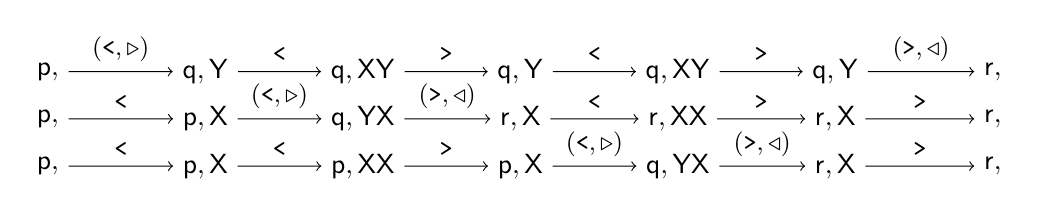
\begin{tikzpicture}[yscale=0.6, node distance=0.5em]
		%		\node[white] (n0) at (0,5) {0};
%		\node (n1) at (2,4.5) {1};
%		\node (n2) at (4,4.5) {2};
%		\node (n3) at (6,4.5) {3};
%		\node (n4) at (8,4.5) {4};
%		\node (n5) at (10,4.5) {5};
%		\node (n6) at (12,4.5) {6};
%		%		
		%		\node[below=of n0,white] (l0) {$\texttt{<}$};
		%		\node[below=of n1] (l1) {$\texttt{<}$};
		%		\node[below=of n2] (l2) {$\texttt{<}$};
		%		\node[below=of n3] (l3) {$\texttt{>}$};
		%		\node[below=of n4] (l4) {$\texttt{<}$};
		%		\node[below=of n5] (l5) {$\texttt{>}$};
		%		\node[below=of n6] (l6) {$\texttt{>}$};
		
		\node (q11) at (1, 3) {${\sf p}, \eps$};
		\node (q12) at (3, 3) {${\sf q}, {\sf Y}$};
		\node (q13) at (5, 3) {${\sf q}, {\sf X}{\sf Y}$};
		\node (q14) at (7, 3) {${\sf q}, {\sf Y}$};
		\node (q15) at (9, 3) {${\sf q}, {\sf X}{\sf Y}$};
		\node (q16) at (11, 3) {${\sf q}, {\sf Y}$};
		\node (q17) at (13, 3) {${\sf r}, \eps$};
		
		\draw[->] (q11) to node [above] {\small$(\texttt{<},\triangleright)$} (q12);
		\draw[->] (q12) to node [above] {\small$\texttt{<}$} (q13);
		\draw[->] (q13) to node [above] {\small$\texttt{>}$} (q14);
		\draw[->] (q14) to node [above] {\small$\texttt{<}$} (q15);
		\draw[->] (q15) to node [above] {\small$\texttt{>}$} (q16);
		\draw[->] (q16) to node [above] {\small$(\texttt{>},\triangleleft)$} (q17);
		
		\node (q21) at (1, 2) {${\sf p}, \eps$};
		\node (q22) at (3, 2) {${\sf p}, {\sf X}$};
		\node (q23) at (5, 2) {${\sf q}, {\sf Y}{\sf X}$};
		\node (q24) at (7, 2) {${\sf r}, {\sf X}$};
		\node (q25) at (9, 2) {${\sf r}, {\sf X}{\sf X}$};
		\node (q26) at (11, 2) {${\sf r}, {\sf X}$};
		\node (q27) at (13, 2) {${\sf r}, \eps$};
		
		\draw[->] (q21) to node [above] {\small$\texttt{<}$} (q22);
		\draw[->] (q22) to node [above] {\small$(\texttt{<},\triangleright)$} (q23);
		\draw[->] (q23) to node [above] {\small$(\texttt{>},\triangleleft)$} (q24);
		\draw[->] (q24) to node [above] {\small$\texttt{<}$} (q25);
		\draw[->] (q25) to node [above] {\small$\texttt{>}$} (q26);
		\draw[->] (q26) to node [above] {\small$\texttt{>}$} (q27);
		
		\node(q31) at (1, 1) {${\sf p}, \eps$};
		\node (q32) at (3, 1) {${\sf p}, {\sf X}$};
		\node (q33) at (5, 1) {${\sf p}, {\sf X}{\sf X}$};
		\node (q34) at (7, 1) {${\sf p}, {\sf X}$};
		\node (q35) at (9, 1) {${\sf q}, {\sf Y}{\sf X}$};
		\node (q36) at (11, 1) {${\sf r}, {\sf X}$};
		\node (q37) at (13, 1) {${\sf r}, \eps$};
		
		\draw[->] (q31) to node [above] {\small$\texttt{<}$} (q32);
		\draw[->] (q32) to node [above] {\small$\texttt{<}$} (q33);
		\draw[->] (q33) to node [above] {\small$\texttt{>}$} (q34);
		\draw[->] (q34) to node [above] {\small$(\texttt{<},\triangleright)$} (q35);
		\draw[->] (q35) to node [above] {\small$(\texttt{>},\triangleleft)$} (q36);
		\draw[->] (q36) to node [above] {\small$\texttt{>}$} (q37);
	\end{tikzpicture}
\end{center}
	Then the reader can check that the output set of running $\cT$ over $w$ is:
	$$
	\sem{\cT}(w) = \big\{(\, \triangleright, 1)(\triangleleft, 6),  \ (\triangleright, 2)(\triangleleft, 3),  \ (\triangleright, 4)(\triangleleft, 5)\, \big\}.
	$$
\end{example}


Strictly speaking, our definition of \vpann is richer than the one studied in~\cite{FiliotRRST18}. In our definition of \vpann each output element is a tuple  $(\oout,i)$ where $\oout$ is the symbol and $i$ is the output position, where for a standard VPT~\cite{FiliotRRST18} an output element is just the symbol $\oout$. 
The extension presented here is indeed important for practical applications like in document spanners~\cite{FlorenzanoRUVV20,AmarilliBMN19} or in XML query evaluation~\cite{BarYossefFJ05, ShalemB08}, as we show next.

\paragraph{Expressiveness of \vpannnames} How useful are \vpann as a computational model for representing queries over nested words? To motivate this question, recall the XPath query $\cQ = \texttt{//a/b}$ presented in the introduction, whose outputs are all pairs of nested tags \texttt{<b/>} and \texttt{<b/>} inside some nested tags \texttt{<a/>} and \texttt{<a/>}. In Figure~\ref{nested:fig-xpath-vpt-small} we show a \vpann equivalent to $\cQ$. The \vpann processes an XML document by moving non-deterministically from $q_0$ to $q_1$ when it reads an open tag \texttt{<a>} and then to $q_2$ when it reads an open tag \texttt{<b>} and marks it with $\downarrow$. Then it moves to $q_3$ when it reads the matching close tag \texttt{<b/>} marking it with $\downarrow$, and it moves to an accepting state when it reads the corresponding close tag \texttt{<a/>}. The reader can easily check that this \vpann marks all pairs of $b$-tags satisfying $\cQ$.  

%!TEC root = ../main/main.tex

\begin{figure}[t]
	\centering
	
	\begin{tikzpicture}[scale=0.7,->,>=stealth',shorten >=1pt,auto,node distance=2cm,thick,state/.style={circle,draw}, color=black, initial text= {},
		initial distance= {5mm}]
		%\node[state,draw=none,scale=0.1] (in) at (-1,0) {};
		\node[state,initial] (q0) at (0,0) {$q_0$};
		\node[state] (q2) at (4,0) {$q_1$};
		\node[state] (q4) at (8,0) {$q_2$};
		\node[state] (q6) at (12,0) {$q_3$};
		\node[state, accepting] (q8) at (16,0) {$q_4$};
		%\draw (in) to (q0);
		
		\draw (q0) to[loop above] node {$\opS / {\sf C}$} (q0);
		\draw (q0) to[loop below] node {$\clS\,\! ,\,\! {\sf C}$} (q0);
		
		\draw (q0) to node [above] {$\op{a} / {\sf A}$} (q2);
		
		\draw (q2) to[loop above] node {$\opS / {\sf C}$} (q2);
		\draw (q2) to[loop below] node {$\clS\,\! ,\,\! {\sf C}$} (q2);
		
		\draw (q2) to node [above] {$\op{b} / {\sf B} \, : \ \, \downarrow$} (q4);
		
		\draw (q4) to[loop above] node {$\opS / {\sf C}$} (q4);
		\draw (q4) to[loop below] node {$\clS\,\! ,\,\! {\sf C}$} (q4);
		
		\draw (q4) to node [above] {$\cl{b}\, ,\,\! {\sf B} \, : \ \, \downarrow$} (q6);
		
		\draw (q6) to[loop above] node {$\opS / {\sf C}$} (q6);
		\draw (q6) to[loop below] node {$\clS\,\! ,\,\! {\sf C}$} (q6);
		
		\draw (q6) to node [above] {$\cl{a} \, ,\,\!  {\sf A}$} (q8);
		
		\draw (q8) to[loop above] node {$\opS / {\sf C}$} (q8);
		\draw (q8) to[loop below] node {$\clS\,\! ,\,\! {\sf C}$} (q8);
		
	\end{tikzpicture}
	
	\caption{A \vpann implementing the CPath query $\cQ = \texttt{//a/b}$. Its input alphabet consists of the sets $\opS$ and $\clS$ of open and closed tags, respectively, $\{{\sf A}, {\sf B}, {\sf C}\}$ is the stack alphabet, and $\{\downarrow\}$ is the output alphabet.}
	
	\label{nested:fig-xpath-vpt-small}
\end{figure}


As in the previous example, one could ask whether \vpann can encode every XPath query or any other query language over nested documents (e.g., JSON). To answer this question, we study the expressiveness of \vpann by comparing it to MSO over nested words. We show that \vpann is equally expressive to MSO over nested words with 
open MSO variables. Given that fragments of query languages over nested documents (e.g., navigational XPath~\cite{CateM07}, JSON Navigational Logic~\cite{BourhisRV20}) are included in MSO logics, this result shows that \vpann is a useful computational model to express query evaluation problems over nested documents. We continue this section by defining MSO over nested words in order to state and prove the main result of the chapter.

In~\cite{AlurM04}, it was shown that VPA describe the same class of queries as MSO over nested words, called $\msom$.
Formally, fix a structured alphabet $\Sigma$ and let $w \in \wnS$ be a word of length~$n$. 
We encode $w$ as a \emph{logic structure}:
$$
\big(\, A, \, \leq,\, \{P_a\}_{a\in\Sigma}, \, \sf{match} \, \big)
$$
where $A = [1,n]$ is the domain, $\leq$ 
is the total order over $[1, n]$, each $P_a$ is a unary predicate encoding the appearance of letter $a \in \Sigma$ such that $P_a = \{i \mid w[i] = a\}$, and $\sf{match}$ is a binary relation over~$[1,n]$ that corresponds to the matching relation of open and close symbols. Formally, for every $i, j \in A$, $\textsf{match}(i, j)$ is true if, and only if, $w[i]$ is an open symbol and $w[j]$ is its matching close symbol.
%By some abuse of notation, we also use $w$ to denote its corresponding logical structure. 
Then, \emph{an $\msom$ formula $\varphi$ over $\Sigma$} is given by the following syntax:
\[
\ \ \ \ \ \ \, \varphi \ :=\ P_a(x) \ \mid\  x \in X \ \mid \ x \leq y \ \mid \ \textsf{match}(x, y) \ \mid \ \neg \varphi \ \mid \ \varphi \vee \varphi \ \mid \ \exists x.\varphi \ \mid \ \exists X.\varphi 
\]
where $a\in\Sigma$, $x$ and $y$ are first-order variables and $X$ is a monadic second order (MSO) variable.
We will use $\bar{x}$ as a shorthand for a list of first-order variables $x_1,\ldots,x_{\ell}$ and $\bar{X}$ as a shorthand for a list of MSO variables $X_1,\ldots,X_m$.
Then, we can write $\varphi(\bar{x}, \bar{X})$ to denote an $\msom$ formula $\varphi$ where $\bar{x}$ and $\bar{X}$ are the free variables of $\varphi$. By some abuse of notation, we will also use $\bar{x}$ and $\bar{X}$ as sets and write $\bar{x} \cup \bar{X}$ to denote the union of $\bar{x}$ and $\bar{X}$.

An \emph{assignment} $\sigma$ for $w$ is a function $\sigma\colon \bar{x}\cup \bar{X}\to 2^{[1,n]}$ such that $|\sigma(x)| = 1$ for every $x \in \bar{x}$. Here, we treat first-order variables as a special case of MSO variables. 
As usual, we denote by $\textsf{dom}(\sigma) = \bar{x}\cup \bar{X}$ the domain of the function $\sigma$. 
Then we write $(w, \sigma) \models \varphi(\bar{x}, \bar{X})$ when $\sigma$ is an assignment over $w$, $\textsf{dom}(\sigma) = \bar{x}\cup \bar{X}$, and $w$ satisfies $\varphi(\bar{x}, \bar{X})$ when each variable in $\bar{x}\cup \bar{X}$ is instantiated by $\sigma$ (see~\cite{libkin2004elements} for the formal semantics of MSO). 
Given a formula $\varphi(\bar{x},\bar{X})$, we define: 
$$
\sem{\varphi}(w) \ = \ \{\sigma \mid (w, \sigma) \models \varphi(\bar{x},\bar{X})\}.
$$ 
For the sake of simplification, from now on we will only use $\bar{X}$ to denote the free variables of $\varphi(\bar{X})$ and use $X \in \bar{X}$ for a first-order or monadic second-order variable.

Given an assignment $\sigma$ over $w$, we can represent $\sigma$ as a sequence of annotations and positions as follows. First, define the \emph{support} of $\sigma$, denoted by $\textsf{supp}(\sigma)$, as the set of positions mentioned in $\sigma$; formally, $\textsf{supp}(\sigma) = \{i \mid \exists X \in  \textsf{dom}(\sigma)\text{ such that } i \in  \sigma(X)\}$. 
Next, assume that $\textsf{supp}(\sigma) = \{i_1,\ldots, i_m\}$ such that $i_j < i_{j+1}$ for every $j < m$. 
Then, we define the \emph{sequence encoding} of $\sigma$ as:
$$
\textsf{enc}(\sigma) \ = \ (\bar{X}_1, i_1) \, (\bar{X}_2, i_2) \, \ldots \, (\bar{X}_m, i_m)
$$
such that $\bar{X}_j = \{X \in \textsf{dom}(\sigma) \mid i_j \in \sigma(X)\}$ for every $j \leq m$. 
In other words, we represent $\sigma$ as an increasing sequence, where each position is labeled with the variables of $\sigma$ where it belongs.

We can now precisely state the equivalence between VPAnn and queries defined by MSO over nested words. Fix a structured alphabet $\Sigma$ and a set of MSO variables $\bar{X}$. We say that a \vpann~$\cT$ with output alphabet $2^{\bar{X}}$ \emph{is equivalent to} an $\msom$ formula $\varphi(\bar{X})$, denoted by $\cT \equiv \varphi$, if, and only if, $
\sem{\cT}(w) = \{\textsf{enc}(\sigma)\mid \sigma\in\sem{\varphi}(w)\}
$ 
for every $w\in \wnS$. In other words, the outputs of $\cT$ are equivalent to the satisfying assignments of $\varphi$ encoded as sequences. 
\begin{proposition}
	For any $\msom$ formula $\varphi(\bar{X})$ there exists a \vpann $\cT$ with output alphabet~$2^{\bar{X}}$ such that $\cT \equiv \varphi$, and conversely. 
\end{proposition}
\begin{proof}
	The following proof is largely based on the proof of Theorem 4 in~\cite{AlurM04}.
	We start by showing how to convert a $\msom$ formula $\varphi(\bar{X})$ into an equivalent \vpann $\cT$. For this, we can follow the exact same argument as the {\em if} direction of the proof in~\cite{AlurM04} and assume we can obtain a VPA $\cA_\varphi$ over the input alphabet $\Sigma^{\bar{X}} = \Sigma \times 2^{\bar{X}}$ whose language is the set of words which encode a valuation $\sigma$ of $\bar{X}$ along with a word $w$ for which $(w, \sigma)\models\varphi(\bar{X})$. 
	We define a straightforward transformation from $\cA_\varphi$ to $\cT$ as follows. Let $t$ be a transition in $\cA_\varphi$ and let $(a, V)$ be its input symbol with $V \in 2^{\bar{X}}$. If $V\neq\emptyset$ the corresponding transition $t'$ in $\cT$ is kept the same, except it has an input symbol $a$, and an output symbol $V$, and if $V = \emptyset$, then $t'$ is obtained by simply replacing $(a, V)$ by $a$.
	One can easily check that $\cT \equiv \varphi$, proving the first direction.
	
	To prove the other direction, we can convert $\cT$ into a VPA $\cA_\cT$ with input alphabet $\Sigma^{\bar{X}}$ in the opposite way and use the result of~\cite{AlurM04} itself to obtain a $\msom$ formula with no free variables $\varphi'$ over the same input alphabet. We replace any instance of $P_{(a, V)}(x)$ in $\varphi$ by the expression $P_a(x) \wedge \bigwedge_{X\in V}x\in X\wedge \bigwedge_{X\in\bar{X}\setminus V}x\not\in X$ to obtain a formula $\varphi(\bar{X})$ over $\Sigma$ which proves the statement.
\end{proof}

We conclude that \vpann has the same expressive power as MSO over nested words, which implies that \vpann can represent the navigational fragments of languages like XPath and JSON Navigational Logic subsumed by MSO. In the next section, we complement this result by stating our main algorithmic results regarding the streaming evaluation of \vpann. Before that, we introduce a class of \vpannnames{} that will be crucial for our algorithmic results.

\paragraph{Deterministic and unambiguous \vpannnames}
We say that a \vpann $\cT = (Q, \Sigma, \Gamma, \oalph, \Delta, \qinit, F)$ is \emph{input/output deterministic} (I/O-deterministic for short)
 if $|\qinit| = 1$ and $\Delta$ is a partial function of the form:
%$$
%\Delta: (Q\times(\opS \times \oalph\cup\opS)\to Q\times \Gamma) \cup 
%(Q\times(\clS\times \oalph\cup \clS)\times\Gamma \to Q) \cup
%(Q\times(\noS\times \oalph\cup\noS) \to Q).
%$$
$$
\renewcommand{\arraystretch}{1.2}
\begin{array}{rcl}
	\Delta & \subseteq & 
	Q \times \big(\opS \cup (\opS \!\times \oalph)\big) \to Q \times \Gamma \ \ \ \cup \\
	& & Q \times \big(\clS  \cup  (\clS \!\times \oalph)\big) \times \Gamma \to Q \ \ \ \cup  \\
	& & Q \times \big(\noS  \cup  (\noS \!\times \oalph)\big) \to Q
\end{array}
$$
%for each triple $(p, a, \oout) \in Q \times \opS \times \oalph$,  there is at most one tuple $(q, \gamma) \in Q \times \Gamma$ such that $(p, a, \oout, q, \gamma)\in\Delta$, 
%for each tuple $(p, a, \oout, \gamma)\in Q \times \clS \times \oalph \times \Gamma$ there is at most one $q\in Q$ such that $(p, a, \oout, \gamma, q)\in\Delta$, 
%and for each triple  $(p, a, \oout) \in Q \times \noS \times \oalph$ there is at most one $q\in Q$ such that $(p, a, \oout, q) \in \Delta$. 
Also, we say that $\cT$ is \emph{input/output unambiguous} (I/O-unambiguous for short) if for every $w\in \wnS$ and every $\mu \in \sem{\cT}(w)$ there is exactly one accepting run $\rho$ of $\cT$ over $w$ such that $\mu = \out(\rho)$. 

Notice that an I/O-deterministic \vpann is also I/O-unambiguous. 
Intuitively, a \vpann is I/O-deterministic (I/O-unambiguous) if, given the input word and a sequence of annotations, the automaton behaves in a deterministic (unambiguous, resp.) manner. 
The definition is in line with the notion of I/O-deterministic variable automata of~\cite{FlorenzanoRUVV20} and I/O-unambiguous is a generalization of this idea that is enough for the purpose of our enumeration algorithm. 

In the next result, we show that for every \vpann $\cT$ there exists an equivalent I/O-deterministic \vpann and, therefore, an equivalent I/O-unambiguous \vpann. 

\begin{proposition} \label{nested:vpawo:det}
	For every \vpann $\cT$ there exists an I/O-deterministic \vpann $\cT'$ of size $\cO(2^{|Q|^2|\Gamma|})$ such that $\br{\cT}(w) = \br{\cT'}(w)$ for every $w\in\wnS$.
\end{proposition}
\begin{proof}
	
Let $\cT = (Q, \Sigma, \Gamma, \oalph, \Delta, \qinit, F)$.
	For the sake of presentation, assume that $\Delta$ contains only transitions with an output symbol, the proof can be extended straightforwardly to include transitions with no output symbol.
	We will construct an I/O-deterministic \vpann $\cT' = ( Q', \Sigma, \Gamma', \oalph, \delta^\dets, S_{I}, F')$ as follows.
	Let $Q' = 2^{Q\times Q}$ and $\Gamma' = 2^{Q\times\Gamma\times Q}$. 
	Let $S_I = \{(q,q)\mid q\in \qinit\}$ and let $F' = \{S\mid (p,q)\in S\text{ for some }p\in I \text{ and } q\in F \}$. 
	Let $\delta$ be defined as follows:
	\begin{itemize}
		\item For $\op{a}\in \opS$ and $\oout\in\Omega$, $\delta(S,\op{a},\oout) = (S',T)$, where:
		\begin{align*}
			T &= \{(p,\gamma,q)\mid (p,p')\in S \text{ and } (p',\op{a},\oout,\gamma,q)\in\Delta\text{ for some }q\in Q \},\\
			S'&= \{(q,q)\mid(p,p')\in S\text{ and }(p',\op{a},\oout,\gamma,q)\in\Delta\text{ for some }p,p'\in Q \text{ and } \gamma\in\Gamma\}
		\end{align*}
		\item For $\cl{a}\in\clS$ and $\oout\in\Omega$, $\delta(S,\cl{a},\oout,T) = S'$ where, if $T\subseteq Q\times\Gamma\times Q$, then: 
		\begin{align*}
			S' &= \{(p,q)\mid(p,\gamma,p')\in T\text{ and }(p',q')\in S\text{ and }(q',\cl{a},\oout,\gamma,q)\in\Delta\ \ \ \ \ \ \ \ \ \ \ \\ &\ \ \ \ \ \ \ \ \ \ \ \ \ \ \ \ \ \ \ \ \ \ \ \ \ \ \ \ \ \ \ \ \ \ \ \ \ \ \ \ \ \ \ \ \ \ \ \ \ \ \ \ \ \text{ for some }p',q'\in Q,\gamma\in\Gamma\},
		\end{align*}
		\item For $a\in\noS$ and $\oout\in\Omega$, $\delta(S,a,\oout) = S'$ where:
		\begin{align*}
			S' &= \{(q,q'')\mid (q,q')\in S\text{ and }(q',a,\oout,q'')\in\Delta\text{ for some }q'\in Q\}.
		\end{align*}
	\end{itemize}
	One can immediately check that this automaton is I/O-deterministic since the transition relation is given as a partial function.
	
	We will prove that $\cT$ and $\cT'$ are equivalent by induction on well-nested words. To aid our proof, we will introduce a couple of ideas. First, we extend the definition of a run to include sequences that start on an arbitary configuration. Also, given a run 
	$$
	\rho = (q_1, \sigma_1) \xrightarrow{b_1} (q_2, \sigma_2) \xrightarrow{b_2} \cdots  \xrightarrow{b_n} (q_{n+1}, \sigma_{n+1}),
	$$
	\noindent and a span $\spanc{i}{j}$, define a subrun of $\rho$ as the subsequence
	$$
	\rho\spanc{i}{j} = (q_i, \sigma_i) \xrightarrow{b_{i}} (q_{i+1}, \sigma_{i+1}) \xrightarrow{b_{i+1}} \cdots  \xrightarrow{b_{j-1}} (q_j, \sigma_j).
	$$
	
	In this proof, we only consider subruns such that $w\spanc{i}{j} = s_{i}s_{i+1}\cdots s_{j-1}$ is a well-nested word. 
	A second definition we will use is that of a \vpann with arbitrary initial states. 
	Formally, let $q\in Q$. 
	We define $\cT_{q}$ as the \vpann that simulates $\cT$ by starting on the configuration $(q,\eps)$. 
	Note that for a run $\rho = (q_1, \sigma_1) \xrightarrow{b_1} \cdots  \xrightarrow{b_n} (q_{n+1}, \sigma_{n+1})$ of $\cT$ over $w = s_1\cdots s_n$ and a well-nested span $\spanc{i}{j}$, the subrun $\rho\spanc{i}{j}$ is one of the runs of $\cT_{q}$ over $w\spanc{i}{j}$ modulo $\sigma_i$, which is present in all of the stacks in $\rho$ as a common suffix.
	
	We shall prove first that $\br{\cT}(w) \subseteq \br{\cT'}(w)$ for every well-nested word $w$. This is done with the help of the following result.
	
	\begin{claim}
		For a well-nested word $w$, output $\mu$, states $p,q\subseteq Q$, and a set $S$ that contains $(p,q)$, if there is a run of $\cT_q$ over $w$ with output $\mu$ such that its last state is $q'$, the (only) run of $\cT'_{S}$ over $w$ with output $\mu$ ends in a state $S'$ which contains $(p,q')$.
	\end{claim}
	
	\begin{proof}
		We will prove the claim by induction on $w$. If $w = \eps$, the proof is trivial since $q = q'$. If $w = a\in\noS$ the proof follows straightforwardly from the construction of $\delta$.
		
		If $w,v\in\wnS$, let $p,q\in Q$, let $S$ be a set that contains $(p,q)$, and let $\rho$ be a run of $\cT_q$ over $wv$ with output $\mu\cdot\kappa$, which ends in a state $q'$, for some $\mu$ and $\kappa$. 
		Our goal is to prove that the run $\rho'$ of $\cT'_S$ over $w\cdot v$ with output $\mu\cdot \kappa$ as output ends in a state that contains $(p,q')$. 
		Let $n = \vert w\vert$, $m = \vert v \vert$, and let $q^w$ be the last state of the subrun $\rho[1,n+1\rangle$. 
		Consider as well $\rho[n+1,n+m+1\rangle$, which is a run of $\cT_{q^w}$ over $v$ with output $\kappa$ that ends in $q'$. 
		From the hypothesis two conditions follow: 
		(1) In the run of $\cT'_S$ over $w$ with output $\mu$, the last state $S'$ contains $(p,q^w)$, and 
		(2) in the run of $\cT'_{S'}$ over $v$ that has $\kappa$ as output the last state contains $(p,q')$. 
		It can be seen that $\rho'$ is the concatenation of these two runs, so this proves the claim.
		
		If $w\in\wnS$, $\op{a}\in\opS$, $\cl{b}\in\clS$, let $p,q\in Q$, $S$ be a set that contains $(p,q)$, and let $\rho$ be a run of $\cT_q$ over $\op{a}w\cl{b}$ with output $(\oout_1, 1)\mu(\oout_2, n+2)$ for some $\mu\in\oalph^*$, $\oout_1,\oout_2\in\oalph$, where $n = |w|$. 
		Let $q, q_2, \ldots, q_{n+2}, q_{n+3}$ be the states of $\rho$ in order. 
		Our goal is to prove that the run $\rho'$ of $\cT'_S$ over $\op{a}w\cl{b}$ with output $(\oout_1, 1)\mu(\oout_2, n+2)$ ends in a state that contains $(p,q_{n+3})$. 
		Let $(q_2,\gamma)$ be the second configuration of $\rho$. 
		This implies that $(q,\op{a},\oout_1,q_2,\gamma)\in\Delta$ and $(q_{n+2},\cl{b},\oout_2,\gamma,q_{n+3})\in\Delta$.
		Let $S'$ and $T$ be such that $\delta(S,\op{a},\oout_1) = (S',T)$.
		Therefore, $(q_2,q_2)\in S'$ and $(p,\gamma,q_2)\in T$.
		Consider the subrun $\rho[2,n+2\rangle$, which can be found as a run of $\cT_{q_2}$ over $w$ with output $\mu$, modulo the stack suffix $\gamma$, and note that it ends in $q_{n+2}$.
		Since $(q_2,q_2)\in S'$, from the hypothesis it follows that the run of $\cT'_{S'}$ over $w$ with output $\mu$ ends in a state $S''$ that contains $(q_2,q_{n+2})$.
		This run starts on the configuration $(S',\eps)$ and ends in $(S'',\eps)$, so a run on the same automaton that starts on $(S',T)$ and reads the same symbols will end in $(S'', T)$, which is the case for the subrun $\rho'[2,n+2\rangle$.
		Therefore, the construction of $\delta$ implies that $(p,q_{n+3})$ is contained in the last state of $\rho'$, which proves the claim.
	\end{proof}
	
	Now let $w$ be a well-nested word and let $\mu \in \br{\cT}(w)$. Let $\rho$ be some accepting run of $\cT$ over $w$ with output $\mu$, and let $p^*\in I$ be its first state and $q^*\in F$ its ending state. 
	Clearly, $\rho$ is also a run of $\cT_p$.
	Now, let us use the claim over the set $S = S_{I}$ and states $p = q = p^*$, using the fact that $(p,p)\in S_{I}$.
	We obtain that the run of $\cT'_{S_I}$ over $w$ with output $\mu$ ends in a state $S'$ which contains $(p,q)$ and so, is it accepting.
	Since $\cT'_{S_I} = \cT'$, this proves that $\br{\cT}(w) \subseteq \br{\cT'}(w)$.
	
	
	To prove that $\br{\cT'}(w) \subseteq \br{\cT}(w)$ we use a similar result:
	
	\begin{claim}
		For a well-nested word $w$, output $\mu$, states $q,p,q'\subseteq Q$, and a set $S$ that contains $(p,q)$, if the run of $\cT'_S$ over $w$ with output $\mu$ ends on a state $S'$ that contains $(p,q')$, then there is a run of $\cT_q$ over $w$ with output $\mu$ such that its last state is $q'$.
	\end{claim}
	\begin{proof}
		We will prove the claim by induction on $w$.
		If $w = \eps$, the proof is trivial since $q = q'$. If $w = a\in\noS$ the proof follows straightforwardly from the construction of $\delta$.
		
		If $w,v\in\wnS$, let $p,q,q'\in Q$, let $S$ be a set that contains $(p,q)$, and let $\rho$ be the run of $\cT'_S$ over $w\cdot v$ with output $\mu\cdot \kappa$, for some $\mu$ and $\kappa$, which ends in a state $S'$ that contains $(p,q')$. 
		Our goal is to prove that there is a run $\rho'$ of $\cT_q$ over $w\cdot v$ with output $\mu\cdot\kappa$ such that its last state is $q'$.
		Let $n = \vert w\vert$, $m = \vert v \vert$, and let $S^w$ be the last state of the subrun $\rho[1,n+1\rangle$. 
		Consider as well $\rho[n+1,n+m+1\rangle$, which is also a run of $\cT'_{S^w}$ over $v$ with output $\kappa$ that ends in $S'$.
		From the construction of $\delta$, it is clear that if a non-empty state $S'$ follows from $S$ in a run of $\cT'$, then $S$ is not empty.
		Let $(p,q^w)\in S^w$.
		From the hypothesis two conditions follow: 
		(1) there is a run $\rho_1$ of $\cT_q$ over $w$ with output $\mu$ such that its last state is $q^w$
		(2) there is a run $\rho_2$ of $\cT_{q^w}$ over $v$ with output $\kappa$ such that its last state is $q'$. 
		We then construct $\rho'$ by concatenating $\rho_1$ and $\rho_2$ which ends in $q'$, and this proves the claim.
		
		If $w\in\wnS$, $\op{a}\in\opS$, $\cl{b}\in\clS$, let $p,q,q'\in Q$, $S$ be a set that contains $(p,q)$, and let $\rho$ be the run of $\cT'_S$ over $\op{a}w\cl{b}$ with output $(\oout_1, 1)\mu(\oout_2, n+2)$ for some $\mu$ and $\oout_1,\oout_2\in\oalph$, where $n = |w|$. 
		Let $S, S_2, \ldots, S_{n+2}, S_{n+3}$ be the states of $\rho$ in order, and suppose there is a pair $(p,q')\in S_{n+3}$.
		Our goal is to prove that there is a run $\rho'$ of $\cT_q$ over $\op{a}w\cl{b}$ with output $(\oout_1, 1)\mu(\oout_2, n+2)$ that ends in $q'$. 
		Let $(S_2,T)$ be the second configuration of $\rho$.
		From the construction of $\delta$, there exist $q_2,q_{n+2}\in Q$ and $\gamma\in\Gamma$ such that $(q_{n+2},\cl{b},\oout_2,\gamma,q_{n+3})\in\Delta$, $(p,\gamma,q_2)\in T$ and $(q_2,q_{n+2})\in S_{n+2}$.
		Since $w$ is well-nested, this $T$ could only have been pushed after a step in the run with label $(\op{a},\oout_1)$, which implies that $(q,\op{a},\oout_1,q_2,\gamma)\in\Delta$. This, in turn, means that $(q_2,q_2)\in S_2$.
		Let us consider the subrun $\rho[2,n+2\rangle$, which is also a run of $\cT'_{S_2}$ over $w$ with output $\mu$ that ends in $S_{n+2}$ modulo the common stack suffix $T$.
		We now have that $(q_2,q_2)\in S_2$ and $(q_2,q_{n+2})\in S_{n+2}$, and so, from the hypothesis it follows that there is a run $\rho''$ of $\cT_{q_2}$ over $w$ with output $\mu$ and ending state $q_{n+2}$.
		In a similar fashion as in the previous claim, we modify the run slightly to obtain one that starts and ends on the stack $\gamma$.
		This new run can be easily extended with the transitions $(q,\op{a},\oout_1,q_2,\gamma),(q_{n+2},\cl{b},\oout_2,\gamma,q_{n+3})\in\Delta$, and as a result, we obtain a run $\rho'$ of $\cT_q$ that fulfils the conditions of the claim.
	\end{proof}
	Now, let $w$ be a well nested word and let $\mu\in \sem{\cT'}(w)$.
	Let $\rho$ be a run of $\cT'$ over $w$ with output $\mu$ that ends in accepting state $F$, and let $p^*\in I$ and $q^*\in F$ be such that $(p^*,p^*)\in I$ and $(p^*,q^*)\in F$. Note that $\cT' = \cT'_{S_I}$, and by using the previous claim with $p = q = p^*$ and $q' = q^*$, we obtain that there is a run of $\cT_{p^*}$ over $w$ with output $\mu$ that ends in state in $q^*$. Clearly, this is also a run of $\cT$, so we obtain that $\mu\in\sem{\cT}(w)$. 
	This proves that $\br{\cT'}(w) \subseteq \br{\cT}(w)$.
	
	We conclude that $\br{\cT}(w) = \br{\cT'}(w)$ for every well-nested word $w$. \hfill \qed
\end{proof}

%The construction of the I/O-deterministic \vpann $\cT'$ from Proposition~\ref{nested:vpawo:det} is similar to the determinization of a VPA we will present in Section~\ref{nested:sec:eval}. Intuitively, to extend this construction from a VPA to a \vpann, one must change the input alphabet from $\opS$ to $\opS \cup (\opS \!\times \oalph)$. 
%Since we will review this construction in Section~\ref{nested:sec:eval}, we move the proof of Proposition~\ref{nested:vpawo:det} to the appendix. 
%Alternatively, the determinization shown in~\cite{AlurM04} is enough to prove the result as well.		

